% !TEX encoding = UTF-8
% !TEX TS-program = pdflatex
% !TEX root = ../tesi.tex
% !TEX spellcheck = it-IT

%**************************************************************
\chapter{Project Development}
\label{cap:project-development}
%**************************************************************

\intro{In this chapter the are described the done point of the project}\\

%**************************************************************
\section{SAM file creation}
At first time, to procede with the project, I've created the SAM file by using the \emph{Burrows-Wheeler Aligner} supplied by BWA.
The software could be found here: \href{http://bio-bwa.sourceforge.net}{http://bio-bwa.sourceforge.net}

The first command necessary for the file creation is:
\\
\\
\verb|bwa index Lactobacillus_casei_genome.fasta|
\\
\\
This command serves to index the fasta genome file. The indexing of the genome's file allows the increasing of the performance during the genome alignment phase.\\

The second typed command is:
\\
\\
\verb|bwa -t 4 mem Lactobacillus_casei_genome.fasta lact_sp.read1.fastq lact_sp.read2.fastq > Lactobacillus_casei_genome.sam|
\\
\\
This command allows the alignment of the two reads files on the reference genome file into a SAM file that servers for the project.\\

There are others different instruments that made this, but BWA should be the best tools specially for the performance.\\

The goal file contains all the informations about the resequenced genome in according with the SAM specifications.
It weight of the file is more or less 890MB.
\newpage

\section{Insertion length}
For this point I wrote an algorithm, that for each row of the SAM file, which contains information about the resequencing, extract the value obtained from :
\\
\\
\verb|abs(POS -PNEXT)|
\\
\\
Where \emph{POS} is the start of the read and \emph{PNEXT} is the start position of the next read.\\
For research fo the insert size length, there are some different opinion that comes from different sources, some of these suggests to use only the \emph{TLEN} field of the SAM file to calculate the insert size length.
\\\\
Once time that I extracted all the insertion length, I plotted all the data in a BatChart trak, as yuo could see here \ref{fig:1}.\\
This trak allows to identify the wrong lectures and the wrong reads.
\\\\
For this trak, a R script was made; from this chart, as I already wrote, is possible to analize the reads that has wrong insert values, which in some cases, is over 2 milion bases long.\\

This error could be partially explained by the multiple alignment of the reads on reference genome.
\newpage
 \begin{figure}[H]
				\centering
				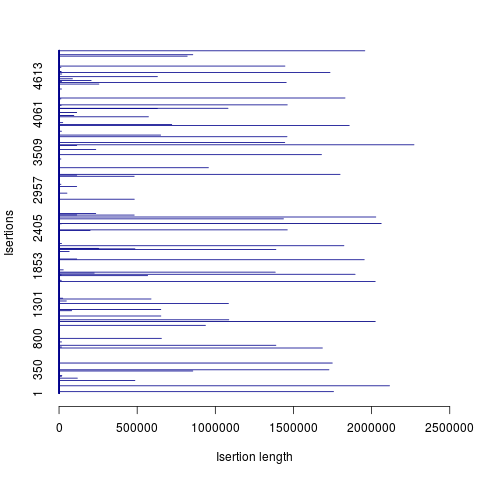
\includegraphics[scale=0.8]{immagini/r.png}
				\caption{Barchart for the isize without exluding errors, the chart include only the first 10.000 reads}\label{fig:1}
				\end{figure}

From this trak, is possibile to see how some read that has the insert lenght longer then 10.000 bases has an error, so for the mean and the standard deviation, this read was be exluded.
Here \ref{fig:2} you could see the trak that exlude the reads with insert equal to or greather then 10.000 bases long. The obtained chart is more right then first chart.
 \begin{figure}[H]
				\centering
				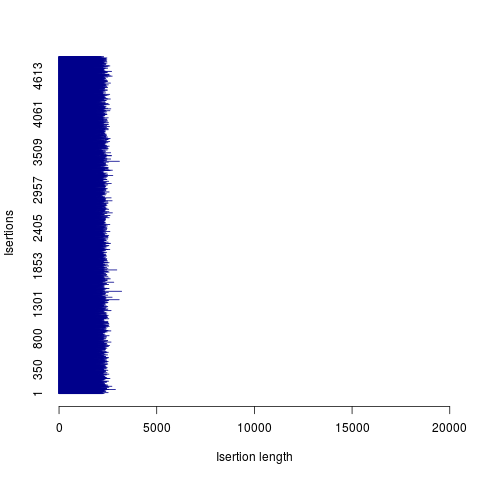
\includegraphics[scale=0.8]{immagini/r1.png}
				\caption{Barchart for the isize without errors}\label{fig:2}
				\end{figure}

The result of mean and standard deviation are:
\begin{itemize}
\item \begin{description}
		\item[MEAN:] 2102
  \end{description}
\end{itemize}

\begin{itemize}
\item \begin{description}
		\item[STD:] 236.85
  \end{description}
\end{itemize}


The result of this point, also, is a csv file that allows to create a barchart with the insertions size with the R script.

\section{Physical Coverage}

The Physical Coverage is calulated by an algorithm really similar to the given Perl script.\\

The mainly reason is the optimization of the algorithm.\\\\

The algorithm, infact, loops on half of reads by checking if the \emph{TLEN} is greather then 0.\\
At first time, I had created an array where each cell was be intialized to 0. 
In each one of these cells, I putted +1 when the index is equal to the read start position, and I putted -1 when the index is equal to the next read start position.\\

Is necessary mentioning which the used reads, are only the right aligned reads, and the filtering of the right-wrong reads is made by checking the \emph{FLAG} field of the SAM file.
\\
The resultant values are putted inside a wig file, called \emph{physical\_coverage.wig}.

After that, the file was loaded onto IGV to show the physical coverage for starting to make hypotesys and analisys about some structural variations.

Some small part of resultant traks produced by the IGV are reported below:

 \begin{figure}[H]
				\centering
				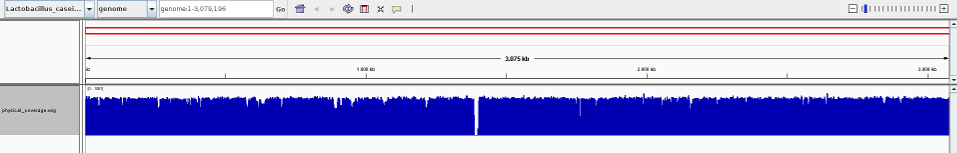
\includegraphics[scale=0.6]{immagini/physical_coverage_1.png}
				\caption{Whole sequence coverage}\label{fig:6}
				\end{figure}


 \begin{figure}[H]
				\centering
				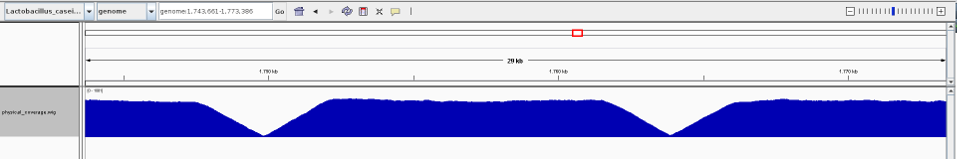
\includegraphics[scale=0.6]{immagini/physical_coverage_2.png}
				\caption{sequence coverage, in the same position the physiscal coverage identify an inversion structural modification}\label{fig:7}
				\end{figure}
				
				
				
 \begin{figure}[H]
				\centering
				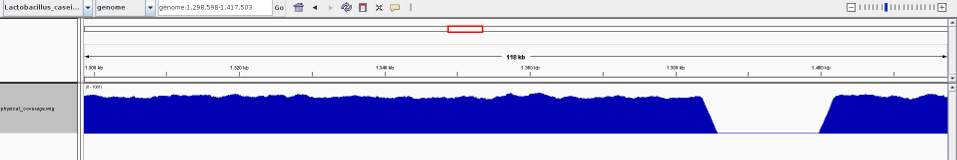
\includegraphics[scale=0.6]{immagini/physical_coverage_3.png}
				\caption{Sequence coverage that identify an structural variation, exactly a long deletation}\label{fig:8}
				\end{figure}				


\section{Sequence Coverage}
The Sequence Coverage is calulated by the algorithm contained inside the SequenceCoverageAlgorithm.py.\\
This algorithm is similar to the physical coverage script's but with the differences who is necessary the read that has positive and negative \emph{TLEN}.\\
As well the Physical coverage, also, this algorithm make a check on the \emph{FLAG} field
\\
\\

At first time, I had created an array where each cell was be intialized to 0.
Then for each cell that has with the index between START to START + sequence lenght, I put +1.
This step is necessary for each compatible reads.\\\\

The resultant values were putted inside a wig file, called \emph{sequeence\_coverage.wig}.

After that the file was loaded onto IGV to show the sequence coverage to help to make hypotesys and analisys about some structural variations.

Some small part of resultant traks produced by the IGV are reported below:


 \begin{figure}[H]
				\centering
				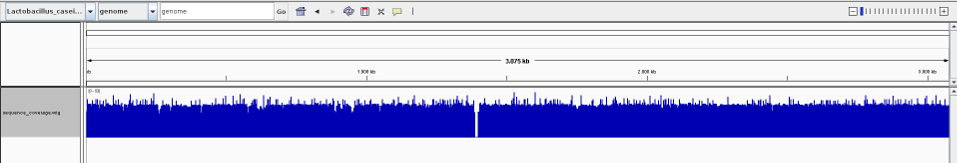
\includegraphics[scale=0.6]{immagini/sequence_coverage_1.png}
				\caption{Whole physical coverage}\label{fig:9}
				\end{figure}


 \begin{figure}[H]
				\centering
				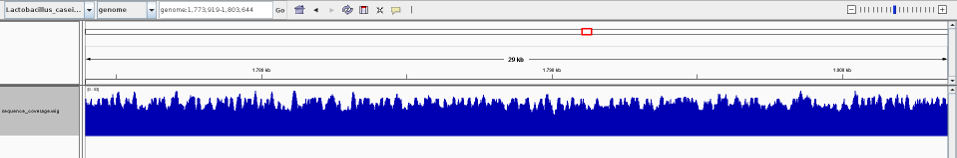
\includegraphics[scale=0.6]{immagini/sequence_coverage_2.png}
				\caption{Physical coverage that identify an structural variation}\label{fig:10}
				\end{figure}
				
				
				
 \begin{figure}[H]
				\centering
				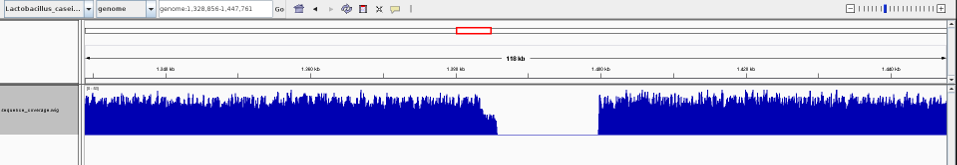
\includegraphics[scale=0.6]{immagini/sequence_coverage_3.png}
				\caption{Physical coverage that identify an structural variation}\label{fig:11}
				\end{figure}	
				
				

\section{Cigar H and S reads}
\label{sec:cigar}
This algorithm allows to find and map the bases that are in the clipped reads.\\
As write in SAM file specifications, there are two kinds of clipping:

\begin{itemize}
\item \begin{description}
		\item[S:] soft clipping (clipped sequences present in SEQ)
  \end{description}
\end{itemize}

\begin{itemize}
\item \begin{description}
		\item[H:] hard clipping (clipped sequences NOT present in SEQ)
  \end{description}
\end{itemize}


This algorithm traks the coverage of the reads with the hard-soft clipping. Below is reported th whole trak of this.
 \begin{figure}[H]
				\centering
				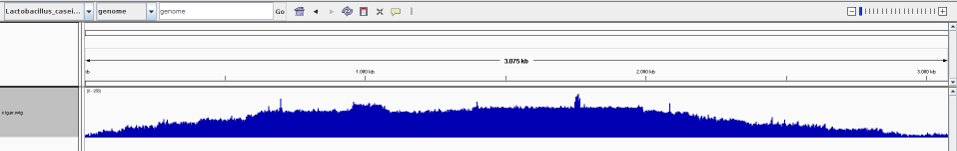
\includegraphics[scale=0.45]{immagini/cigar_coverage_1.png}
				\caption{Whole coverage of the bases involved in a clipping}\label{fig:15}
				\end{figure}	
				
Is interested to see how in corrisponding postion of the structural inversions, the cigar's trak has some peak:

 \begin{figure}[H]
				\centering
				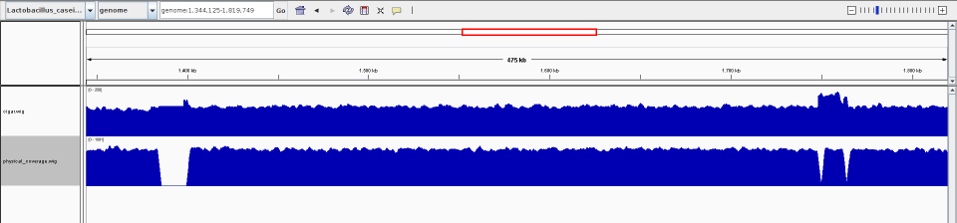
\includegraphics[scale=0.45]{immagini/cigar_coverage_2.png}
				\caption{Cigar coverage and physical coverage that allow to undestand the structural varations}\label{fig:16}
				\end{figure}	
As we can see in the figure \ref{fig:16}, in the proximity of deletetaion and specially in proximity of inversion structural variations, the cigar's trak has peaks; this peaks allow to understand and to confirm the presence of the strutural variations.		

						
\section{Kmers counting}
To start talking about the kmers, is necessay to define what is it.
\begin{quote}
The term k-mer typically refers to all the possible substrings of length k that are contained in a string. In computational genomics, k-mers refer to all the possible subsequences (of length k) from a read obtained through DNA Sequencing
\end{quote}

The algorithm for the kmers analisys is inside the KmersAlgorithm.py.\\
to work, the algorithm expects the kmers length value, many different test was made using 7-mers, 4-mers and 9-mers.\\
The result was be really different and to make some hypotesys or analisys was be necessary plot different barchart by usign some R scripts.\\\\

These traks has allowed to learn and see what are the most, and the less present kmers inside the resequenced genome.\\

The algorithm consider each kmers with the relative opposite, the goal is eliminate the errors that could comes from the "string slicing" from the kmers build.\\\\

The algorithm start from position 0 of each \emph{SEQ} and terminate with the end of \emph{SEQ}.
In each loop made on the SEQ string, the algorithm move the start position from \verb|i| to \verb|i+1| and the end position from \verb|end| to \verb|end+1|.\\
The resultant substring is exactly long how we aspect.\\\\

I reported the traks generated by the different k dimensions below:

 \begin{figure}[H]
				\centering
				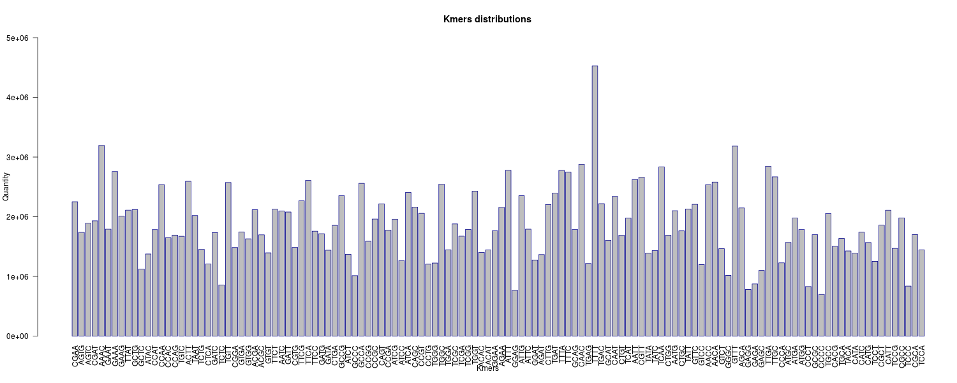
\includegraphics[scale=0.45]{immagini/kmers_4.png}
				\caption{Kmers with k = 4}\label{fig:12}
				\end{figure}


 \begin{figure}[H]
				\centering
				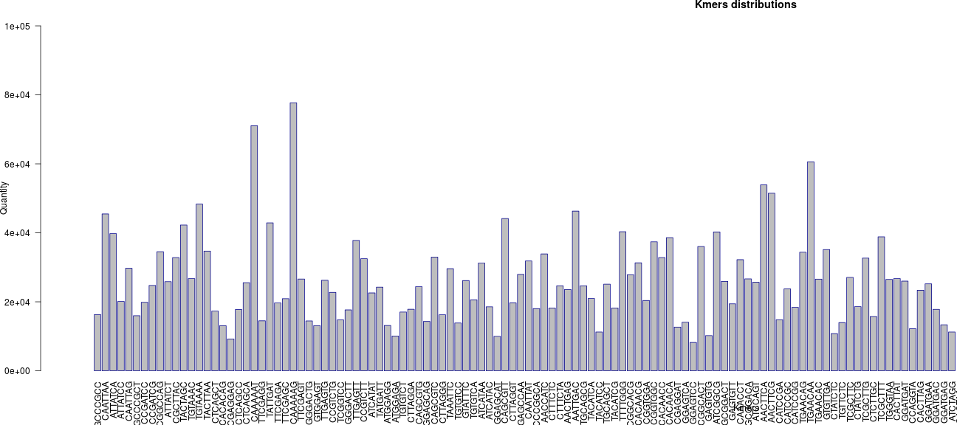
\includegraphics[scale=0.45]{immagini/kmers_7.png}
				\caption{Kmers with k = 7}\label{fig:13}
				\end{figure}
				
				
				
 \begin{figure}[H]
				\centering
				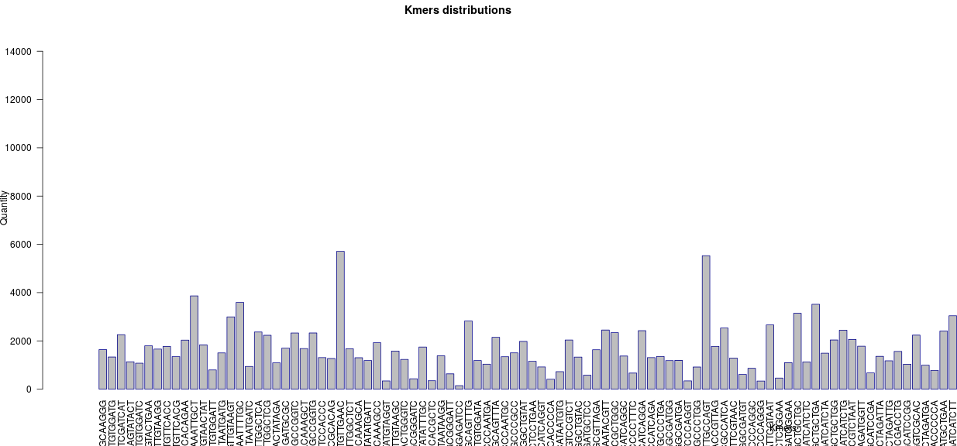
\includegraphics[scale=0.45]{immagini/kmers_9.png}
				\caption{Kmers with k = 9}\label{fig:14}
				\end{figure}	
				
In these traks is simple to see what kmers are more frequent then others, the observation of the kmers and the relative bases should be helpfull for the gene recongition, because should allows the reasearch of a certain protein.\\\\
The result of this algorithm is a csv file that maps kmer name with the kmer frequence				
